%\documentclass[a4paper,10pt]{article}
%\usepackage[utf8]{inputenc}

\documentclass[journal]{IEEEtran}
\usepackage{blindtext}
\usepackage{graphicx}
\usepackage{amsmath}
\usepackage{pdfpages}
\usepackage{hyperref}

\hypersetup{
	colorlinks = true,
	citecolor = {blue},
	urlcolor = {black}
}

\graphicspath{ {Pictures/} }

\markboth{North Dakota State University, December~2015}%
{Shell \MakeLowercase{\textit{et al.}}: Bare Demo of IEEEtran.cls for Journals}

\title{Measuring Transmembrane Potential of Mouse Hypridoma cell culture in Radio Frequency Spectrum}
\author{Andrew Bossert, Christopher Jordan - Denny, Nicolette Lippert}

\begin{document}

\maketitle

\begin{abstract}
This article explores using dielectric spectroscopy in an attempt to measure the trans-membrane potential of synthetic cells in radio frequency spectrum. The purpose of this test is to "mimic" a capacitor with the cell suspension acting as a dielectric. This is a non-invasive way to measure the average membrane potential across your cell suspension and has been proven in \cite{Dielectric Spectroscopy} for frequencies up to \textbf{$10^5 Hz$}.
\end{abstract}

\section{Implications of Membrane Potential}
Although there may be many implications of transmembrane potential at radio frequencies, the focus of this example is in disease models. In the late 1930's it was suggested that a relationship lie between cancer and the bioelectric properties of host tissue. Interestingly, membrane voltage ($V_{mem}$) analysis in many different mammalian cell types reveals that proliferative potential is correlated with unique ranges of $V_{mem}$ : quiescent cells tend to be hyperpolarized, whereas highly plastic cells such as embryonic cells,adult stem cells and tumors cells are depolarized. \cite{TMP-implications}. During the early stages of tumor formation, $V_{mem}$ is a key regulator of the cell cycle and determines the proliferative state of many different kinds of cells. These statements excite the possibility of non-invasive techniques being used to track bioelectric cell states and detection of tumors, or even mitigation of tumor formation by canonical oncogene.

\section{Hypothesis}


\section{Calculating Membrane Potential}
We model the impedance of the cell suspension as a resitor $R = d/\sigma A$ in parallel with a capacitor $C = \epsilon A/d$, where $\sigma$ and $\epsilon$ are the conductivity and dielectric permittivity of the cell suspension and $A$ and $d$ are the surface area of the two disk electrodes and the distance between them. 

\begin{equation}
\label{conductivity}
\sigma(\omega) = Re\frac{d_1-d_2}{A(Z_1^O-Z_2^O)}
\end{equation}

\begin{equation}
\label{permittivity}
\epsilon(\omega) = Im\frac{d_1-d_2}{\omega A(Z_1^O-Z_2^O)}
\end{equation}

Electrode distance variation technique:

\begin{equation}
\begin{aligned}
\label{variation technique derivation}
\mathcal Z_1^S-Z^P &= Z_1^O \\
\mathcal Z_2^S-Z^P &= Z_2^O
\end{aligned}
\end{equation}

\begin{equation}
\label{variation technique}
Z_1^S-Z_2^S = Z_1^O - Z_2^O
\end{equation}

Where $Z^S$ is the sample impedance, $Z^P$ is the unknown polarization impedance, and $Z^O$ is the measured impedance. \\

I have been assured by Dr.Dharmakeerthi Nawarathna that equation (\ref{conductivity}) and equation (\ref{permittivity}) are sufficient in finding the potential of the solution.

\section{Distance Between Plates:}
With regards to near and far field transmission. The most agreed upon definition of near field transmission is less than one wavelength($\lambda$) away \cite{near-far-em}. If we consider a sinusoidal wave traveling at a constant speed, we can calculate wavelength with the following formula \ldots

\begin{equation}
\label{wavelength}
\lambda = \frac{v}{f}
\end{equation}

Where $v$ is the magnitude of the phase velocity and $f$ is the frequency of the sinusoid. It is difficult to determine the phase velocity of our electromagnetic wave while propagating through our cell suspension, but if we consider water, we can make a prediction of the wavelength. The velocity of EM waves is more than 4 orders faster than acoustic waves according to \cite{wave-propagation-water}. Knowing that the speed of sound is $343.2 m/s$ we can say \ldots

\begin{equation}
\label{near-wavelength-water}
\lambda = \frac{343.2 \cdot 4}{10^9} = 1.3728 \times 10^{-6} m
\end{equation}

Water is a good basis for the phase velocity as the cell suspension is made from deonized water and synthetic cells. I used $10^9 Hz$ as our frequency, which is in the radio spectrum. Our micrometer is sensitive to $10\mu m$, thus our test fixture will be capable of measuring only waves 10 times greater than the fundamental wavelength, meaning far field transmissions will be measured. This is a satisfactory result, as the far field is the "real" radio waves, that propagate through space at just about the speed of light \cite{near-far-em}. 

\section{S-Parameters}
At low frequencies it is common to use the transfer and impedance matrices, since this experiment used high frequencies scattering parameters are more preferable. A linear two-port network is used to characterize the equivalent circuit parameters for our experiment. More specifically Scattering parameters are used to relate the outgoing waves $b_1,b_2$ to the incoming waves $a_1,a_2$. The parameters $S_{11},S_{22}$ are the reflection coefficients, or the ratio of the amplitude of the reflected wave to the incident wave. The parameters $S_{21},S_{12}$ are the transmission coefficients, or the amplitude, intensity or total power of a transmitted wave relative to a incident wave (Power of propagation through a medium). As a reminder the incident wave is the wave traveling from source to load, as the reflected wave is the traveling from load to source.

\begin{figure}[h]
\label{Equivalent_Circuit}
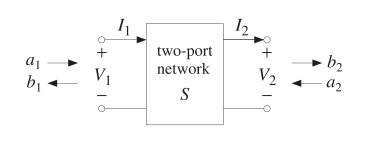
\includegraphics[width=8cm]{two_port.png}
\end{figure}

\begin{figure}[h]
\label{Equivalent_Circuit}
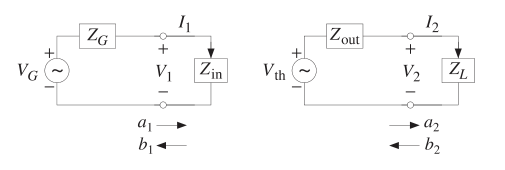
\includegraphics[width=8cm]{Equivalent_Circuit.png}
\end{figure}

\begin{equation}
\label{thevenin-equation-1}
V_{th} = \frac{Z_{21}\cdot V_G}{Z_{11}+Z_{G}}, Z_{th}=Z_{out}=Z_{22}-\frac{Z_{12}\cdot Z_{21}}{Z_{11}+Z_G}
\end{equation}

\begin{equation}
\label{thevenin-equation-1}
Z_{in}=Z_{11}-\frac{Z_{12}\cdot Z_{21}}{Z_{22}+Z_L}
\end{equation}

\begin{equation}
\label{s-conversion}
Z = \frac{Z_O}{D_s}
\begin{bmatrix}
A & 2\cdot S_{12}\\ 
 2\cdot S_{21} & D
\end{bmatrix}
\end{equation}

\begin{align*}
A &= (1+S_{11})(1-S_{22})+S_{12}S_{21}\\
D &= (1-S_{11})(1+S_{22})+S_{12}S_{21}\\
D_s &= det(I-S) = (1-S_{11})(1-S_{22})-S_{12}S_{21}
\end{align*}

\section{Materials}

\begin{figure}[h]
\label{test-fixture}
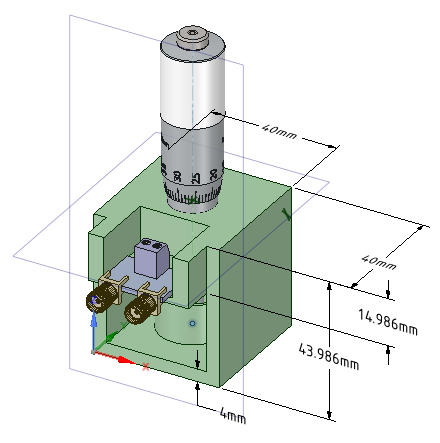
\includegraphics[width=8cm]{Combined_Test_Fixture.png}
\end{figure}

\subsection{Copper Plates}
Two copper plates $3/4 \: inch$ in diameter will be used. One plate will be fixed to the bottom of the beaker and the other is attached to a micrometer. To create the copper plates a hole puncher will be used.

\subsection{Copper Wire Leads}
Two wires will be attached to the copper plates. The wire attached to the fixed bottom plate will be attached to the center and run through the bottom of the test fixture to later be attached to a network analyzer.The second wire will be attached to top plate on one of the edges and run up the side of the beaker to be attached to a network analyzer. These two wires will provide the radio frequency signal and the probes to be attached to a network analyzer.

\subsection{3-D printed Beaker}
A 3-D printed beaker will be made to perfectly fit the test fixture. The beaker will be made of ABS plastic and is used to hold the cell suspension and two copper plates. It will be placed in the center of the Test fixture stand.

\subsection{Micrometer}
A micrometer will be used to adjust the height of one of the copper plates. The micrometer will be attached to the test fixture stand, and the drive of the micrometer will be attached to one of the copper plates. A micrometer cap will be 3-D printed in ABS plastic to perfectly fit the micrometer and later be adhered to the copper plate.

\subsection{Test Fixture Stand}
Provide a base for the beaker as well as an accurate and stable micrometer mount.This item will be 3D printed with ABS plastic.

\subsection{Cells}
SP 2/0 myelomas hypridoma cell line. These are nonadherent cells, and are essentially cancer cells from mice.\cite{mouse-myeloma-hybridoma-strain} They are rated at biosafety level 1. This level is suitable for work involving well-characterized agents not known to consistently cause disease in healthy adult humans, and of minimal potential hazard to laboratory peronnel and the environment. Reasearch with these agents may be performed on standard open laboratory benches without the use of special containment equipment and it is not necessary for Biosafety level 1 labs to be isolated from the general building.\cite{biosafety-levels}

\subsection{Hewlett-Packard 8735E Network Analyzer 30kHz - 6GHz}
Used with this network analyzer was the Agilent 11857D 7mm test port returns($50\Omega$). This network analyzer was used to gather our scattering parameters. This version features the 006 option which give it a 6 GHz upper frequency range.\\
Resolution: $1 Hz$ \\
Stability: typically $\pm7.5 ppm$ \\
Accuracy: $\pm10 ppm$\\
Resolution: $0.05 dB$


\begin{figure}[h]
\label{test-fixture}
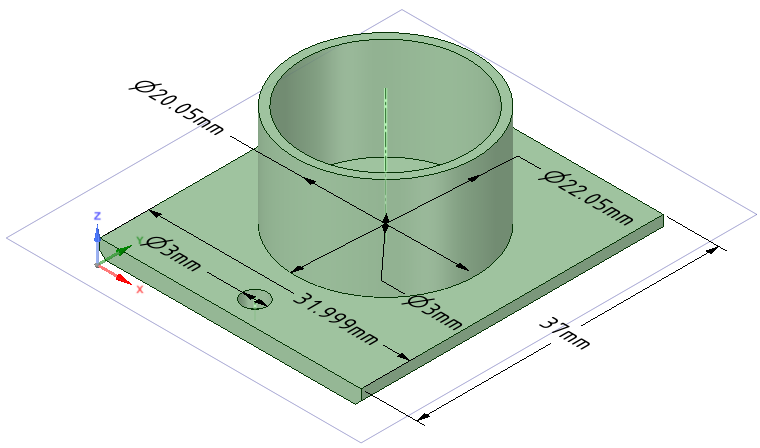
\includegraphics[width=8cm]{Beaker.png}
\end{figure}

\section{Methods}

\subsection{Cell Concentration}
The cell concentration will be measured using a hemocytometer. An example of the process of counting the cells can be seen in figure

\begin{figure}[h]
\label{hemocytometer}
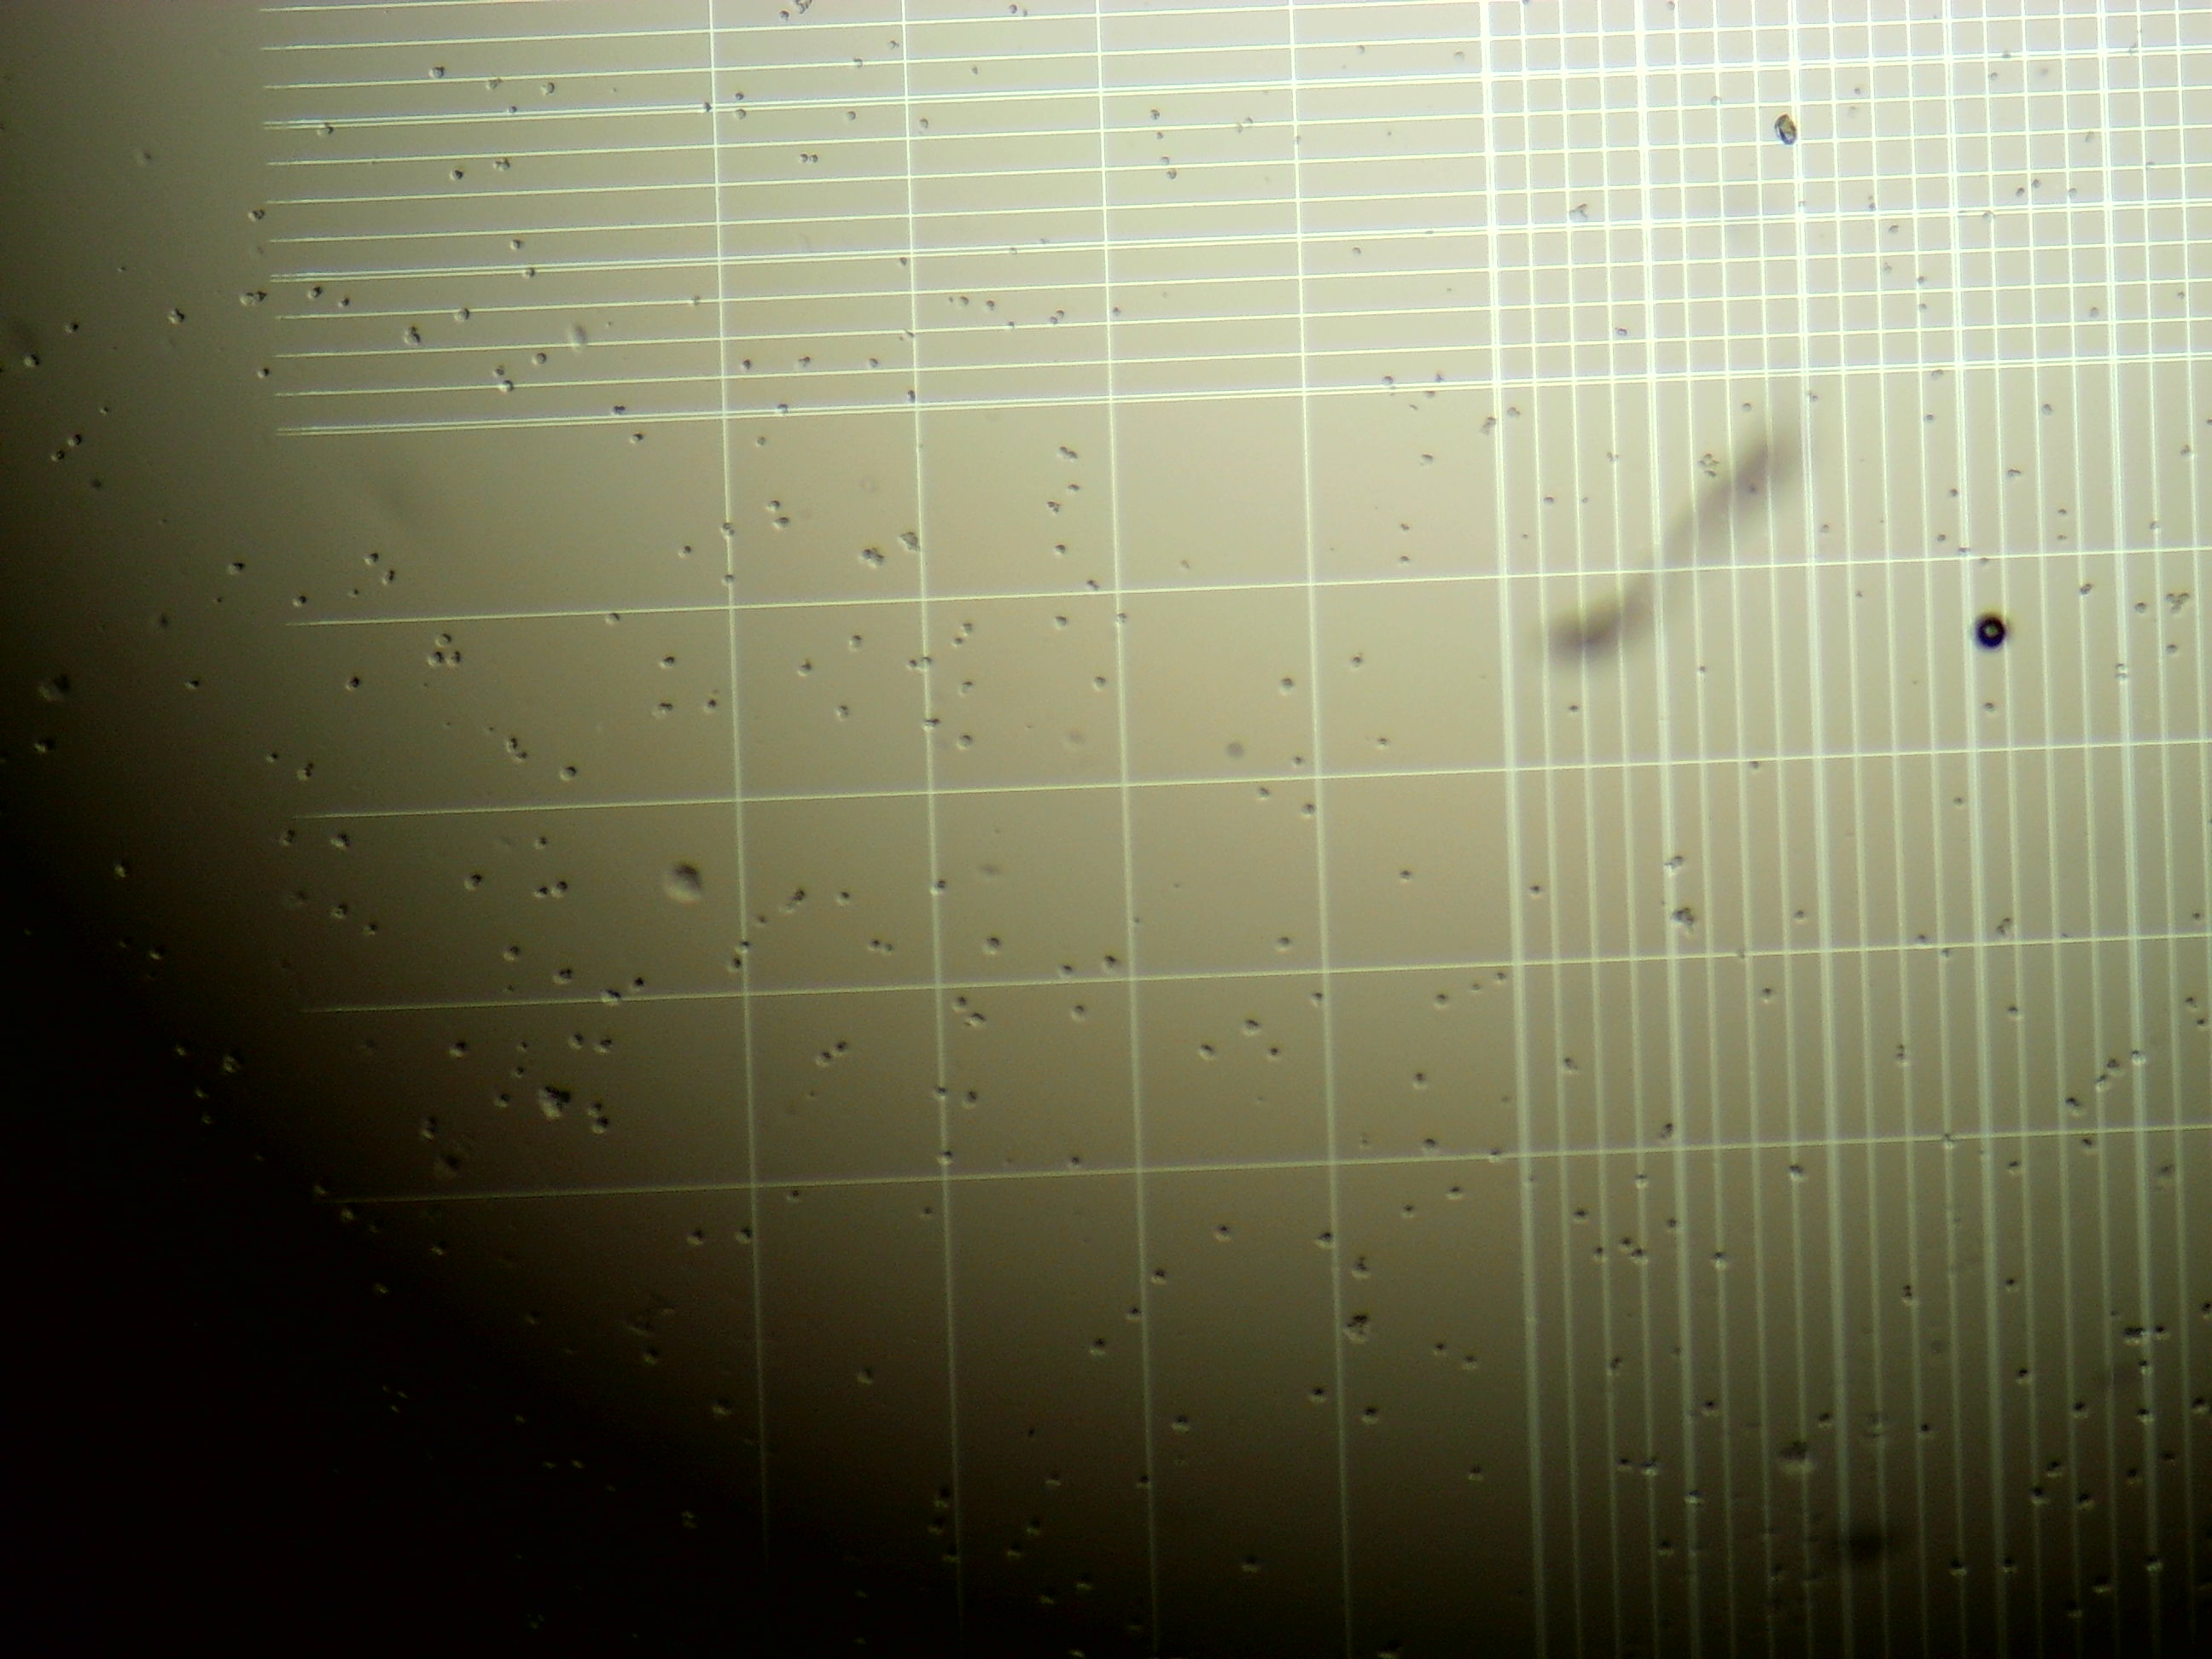
\includegraphics[width=9cm]{hemocytometer.jpg}
\end{figure}

\section{Procedure for splitting cells for regrowth and testing}
\subsection{Tools and Equipment}
\begin{itemize}
\item New cell culture flask
\item Centrifuge
\item 1ml centrifuge vials 
\item Pipette with 10ml graduated tips
\item Bleach
\item Phosphate buffer solution (PBS)
\item Cell food (10\% FBS PFS solution)
\item Vial rack for the centrifuge vials
\item 50ml sealable test tube
\end{itemize}

\subsection{Personal Safety Equipment}
For bio safety level 2, use of hood, gloves, and lab coat for person protection. With the hood shield down, protective eye ware was not needed. The hood should be turned on, and the shield lowered so only your hands can fit underneath it,  before any work with the cells is done. The cells are not to leave the bio safety level 2 lab room.

\subsection{Notes}
\begin{itemize}
\item The cell suspension will become more acidic over time, and thus, the more yellow or orange than dark pink (the color of the cell food).
\item The cells are being kept under conditions of 37 $\circ C$ and 4.9\% CO2 in the incubation chamber when not in use. 
\item The food is being stored in a standard refrigerator in a bio safety lab room.
\item The process does not need to leave the room to be completed.
\end{itemize}

\subsection{Procedure}

\textbf{Centrifuging:}
\begin{enumerate}
\item Remove the flask from the incubation unit and place it in the hood
\item Using the pipettes, put 1 ml of cell solution from the cell culture flask into each of the centrifuge vials until no more solution in the flask. 10 vials should be full.
\item Seal the vials, and evenly distributed them in a centrifuge which is then run at 1.7krpm for 5 min. Once complete, there will be a pellet of cells in the bottom of those vials. If there is an odd number of vials, do not use the odd one, place it aside on the rack for later disposal.
\item Split the vials into two equal groups. One group will be used to create the solution for testing and the other will be used to regrow the cell population.
\end{enumerate}

\textbf{For cell regrowth:}
\begin{enumerate}
\item Siphon off the solution in the vials and put it in the test tube. 
\item Using a new pipette, add 1ml of food to the vials. The tip of the pipette will not touch the cells.
\item Shake the vials to dissolve the pellet.
\item Using a pipette, add the solution of cells and cell food to a new cell culture flask. The flask should be labeled with the type of cells or strain, and what path number they are on.
\item The flask is then sealed, and placed horizontally back in the incubation chamber until this process needs to be repeated.
\end{enumerate}

\textbf{Preparing Cells for testing:}
\begin{enumerate}
\item Repeat step 1 from the Cell regrowth section
\item Using the pipette, add 1 ml of a buffer solution, phosphate saline buffer solution is added to the vials
\item Repeat step 3 of the Cell Regrowth section
\item Using the pipette, the solution can be added as needed to the test fixture. It can also be stored temporarily in test tube or a cell culture flask.
\end{enumerate}

\textbf{For unused centrifuge vials:}
\begin{enumerate}
\item Repeat step 1 from the Cell regrowth section
\item Using the pipette, add 1ml of bleach to the vials
\item Shake the vials to dissolve
\item Using a pipette, the bleach and cell solution is added to the mixture of old cells already in the disposable test tube. 
\end{enumerate}

\textbf{Clean up:} \\
If the disposable test tube has not had bleach added to it, several milliliters should be added to it. The liquid should turn light blue to clear, and now can safely be disposed. All surfaces in the hood and materials that are not disposable should be wiped down with 70\% ether solution. All equipment used that is disposable should disposed of in bio-safe bins which should be located near the hood. 

\section{Conclusion}
The reason for the test fixture is to hold a beaker dish and
  adjust the height between the two parallel copper plates. In order to be as accurate as possible a micrometer will be attached to the top copper plate and then attached to the top of the test fixture. This will allow us to accurately set the parallel plate distance and also change the height as needed. 

\section{Acknowledgement}
The authors would like to acknowledge Daniel Ewert and Jared Hansen for their leadership in this project. A special thanks to Dhamakeerthi Nawarathna for his help in the biology lab.

\begin{thebibliography}{9}

\bibitem{Dielectric Spectroscopy}
C.Prodan,F.Mayo,J.R.Claycomb,J.H.Miller,Jr,M.J.Benedik.
\textit{Low-frequency, low-field dielectric spectroscopy of living cell suspensions}.
Journal of Applied Physics, Volume 95, Number 7, April 2004

\bibitem{wave-propagation-water}
Shan Jiang, Stavros Georgakopoulos.
\textit{Electromagnetic Wave Propagation into Fresh Water}.
Journal of Electromagnetic Analysis and Applications,2011,3,261-266

\bibitem{near-far-em}
Lou Frenzel.
\textit{What is the Difference Between EM Near Field and Far Field}.
Electronic Design, June 8, 2012

\bibitem{TMP-implications}
Brook T.Chernet and Michael Levin
\textit{Transmembrane voltage potential is an essential cellular parameter for the detection and control of tumor development in a Xenopus model}. Disease Models & Mechanisms 6, 595-607 (2013)

\bibitem{biosafety-levels}
Center for Disease Control and Prevention
\textit{Recognizing the Biosafety Levels}.
\url{www.cdc.gov/training/QuickLearns/biosafety/}

\bibitem{mouse-myeloma-hybridoma-strain}
ATCC
\textit{Mouse Myeloma Hybridoma Strain 6C2-4 (PTA-970)}.
American Type Culture Collection

\end{thebibliography}

\end{document}
